\documentclass[aspectratio=169,10pt]{beamer}
\usetheme{Madrid}
\usecolortheme{default}
\usepackage[utf8]{inputenc}
\usepackage[T1]{fontenc}
\usepackage{amsmath}
\usepackage{booktabs}
\usepackage{tikz}
\usetikzlibrary{positioning,arrows.meta}
\setbeamertemplate{navigation symbols}{}

\title[Phantom Dependencies]{Phantom Dependencies}
\subtitle{Package Hallucination in LLM-Generated Python and JavaScript Code\\Across Models, Prompt Languages and Guardrail Prompts}
\author[Rana, Aswal, Trivedi, Shrivastava]{Vansh Rana (590017823) \and Anirudh Singh Aswal (590017310)\\ Hardik Trivedi (590016152) \and Yash Shrivastava (590011391)}
\institute{Research Methodology}
\date{}

\begin{document}

% ---------- Slide 1 ----------
\begin{frame}
\titlepage
\end{frame}

% ---------- Slide 2 ----------
\begin{frame}{Problem and Research Gap}
\begin{columns}[T]
\begin{column}{0.5\textwidth}
\textbf{The problem}
\begin{itemize}
\item LLM coding assistants sometimes import packages that \alert{do not exist}.
\item Attackers register those names on PyPI/npm with malware: \alert{slopsquatting}.
\item Hallucinated names recur, so they are predictable targets.
\item Agentic tools run \texttt{pip}/\texttt{npm install} with no human check.
\end{itemize}
\end{column}
\begin{column}{0.5\textwidth}
\textbf{Prior work}: Spracklen et al.\ (USENIX Sec.\ 2025): 576k samples, 16 models; $\geq$5.2\% (commercial) and 21.7\% (open-weight) hallucination; 43\% recurrence.

\medskip
\textbf{Gaps we address}
\begin{itemize}
\item \textbf{G1} Prompt language: no study of non-English (Hindi) prompts.
\item \textbf{G2} Cheap mitigation: zero-cost guardrail prompt untested.
\item \textbf{G3} Exists $\neq$ safe: need time-anchored registry checks.
\end{itemize}
\end{column}
\end{columns}
\end{frame}

% ---------- Slide 3 ----------
\begin{frame}{Research Questions and Hypotheses}
\begin{columns}[T]
\begin{column}{0.5\textwidth}
\textbf{Research questions}
\begin{itemize}
\item \textbf{RQ1} How often do current LLMs reference non-existent packages?
\item \textbf{RQ2} Effect of model, language, difficulty, recency?
\item \textbf{RQ3} Does a guardrail system prompt reduce it?
\item \textbf{RQ4} Do Hindi prompts change it?
\item \textbf{RQ5} How often do names recur within/across models?
\end{itemize}
\end{column}
\begin{column}{0.5\textwidth}
\textbf{Hypotheses}
\begin{itemize}
\item \textbf{H1} JavaScript $>$ Python
\item \textbf{H2} Hard / recent-library tasks $>$ easy / established
\item \textbf{H3} Open-weight $>$ proprietary
\item \textbf{H4} Guardrail lowers odds (one-sided)
\item \textbf{H5} Hindi raises odds (one-sided)
\item \textbf{H6} Guardrail effect smaller in Hindi
\end{itemize}
\end{column}
\end{columns}
\end{frame}

% ---------- Slide 4 ----------
\begin{frame}{Methodology}
\begin{columns}[T]
\begin{column}{0.48\textwidth}
\textbf{Factorial design}\\
Model (4) $\times$ Prompt (baseline, guardrail) $\times$ Language (English, Hindi)
\begin{itemize}
\item 240 prompts (120 Python, 120 JS) from the public Spracklen et al.\ dataset
\item 1 sample at $T{=}0$ + 5 at $T{=}0.7$
\item $240\times4\times2\times2\times6 = \mathbf{23{,}040}$ generations
\item Hindi via translation + back-translation
\end{itemize}
\end{column}
\begin{column}{0.5\textwidth}
\centering
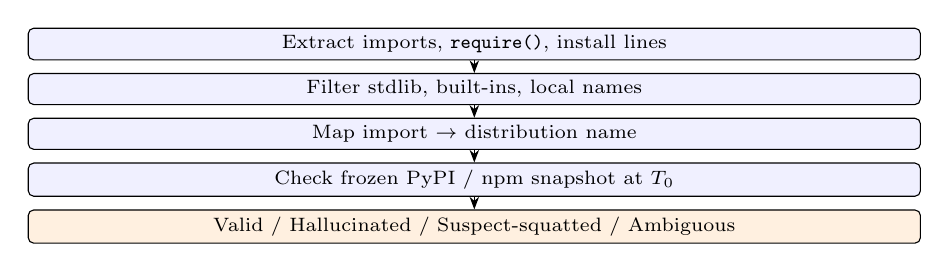
\begin{tikzpicture}[node distance=1.6mm,
  box/.style={draw, rounded corners=2pt, fill=blue!6, align=center, font=\scriptsize, text width=0.92\columnwidth, inner sep=2.5pt},
  arr/.style={-{Stealth[length=1.6mm]}}]
\node[box] (a) {Extract imports, \texttt{require()}, install lines};
\node[box, below=of a] (b) {Filter stdlib, built-ins, local names};
\node[box, below=of b] (c) {Map import $\rightarrow$ distribution name};
\node[box, below=of c] (d) {Check frozen PyPI / npm snapshot at $T_0$};
\node[box, below=of d, fill=orange!12] (e) {Valid / Hallucinated / Suspect-squatted / Ambiguous};
\foreach \x/\y in {a/b,b/c,c/d,d/e} \draw[arr] (\x) -- (\y);
\end{tikzpicture}
\end{column}
\end{columns}
\end{frame}

% ---------- Slide 5 ----------
\begin{frame}{Analysis, Ethics and Expected Contributions}
\begin{columns}[T]
\begin{column}{0.5\textwidth}
\textbf{Analysis}
\begin{itemize}
\item Package- and response-level hallucination rate (Wilson 95\% CI)
\item Repeat rate and cross-model Jaccard overlap
\item Binomial GLMM (\texttt{lme4}), random effects for task and response; Holm correction
\end{itemize}
\textbf{Ethics}
\begin{itemize}
\item No hallucinated names registered by us
\item Malicious names reported to PyPI/npm before release
\end{itemize}
\end{column}
\begin{column}{0.5\textwidth}
\textbf{Expected contributions}
\begin{enumerate}
\item Updated, time-anchored measurement on 2025--26 models
\item First estimate of Hindi vs.\ English prompt effect
\item Evidence on a zero-cost guardrail prompt
\item Open extraction-and-verification pipeline and dataset
\end{enumerate}
\medskip
\textbf{Data:} \url{https://zenodo.org/records/14676377}\\
\textbf{Code:} \url{https://github.com/rvansh0025-glitch/research-methodology-vansh-rana}
\end{column}
\end{columns}
\end{frame}

\end{document}
